\chapter{Ping-Pong-Loopによる固有符号推定}
本章では,4章の検討内容の基礎となる,Ping-Pong-Loop(以下PPL)アルゴリズムについて説明する.

\section{Vector Coding}
最初にVCを説明するにあたって必要なチャネル行列の定義を行った上で,VCの概要について説明する.

\subsection{チャネル行列}
チャネルインパルス応答$h[n]$は以下で与えられている.
\begin{equation}
    h[n] = \left\{
        \begin{array}{ll}
            = 0 & (n<0 \quad or \quad n \geq K) \\
            \neq 0 & (n=0)
        \end{array}
    \right.
\end{equation}
伝送信号系列を$x[n]$とすると,受信信号系列$y[n]$は(3.1)式を用いて,次の畳み込み
演算で与えられる.
\begin{equation}
    y[n] = \sum_{m=0}^\infty h[n-m]x[m]
\end{equation}
送信変調ベクトルをN次の列ベクトル$\bm{X}(=x[0],x[1],\ldots,x[N-1])^T$,チャネル行列を
$\bm{H}$とすると,受信信号ベクトル$\bm{Y}$は(3.2)式を行列表記することで下記のように
与えられる.
\begin{equation}
    \bm{Y} = \bm{HX}
\end{equation}
ここで$\bm{Y}$は$M(=N+K-1)$次の列ベクトル$(=y[0],y[1],\ldots,y[M-1])^T$で,チャネル歪み
の影響でN次からM次になっている.Kはパス数である.$\bm{H}$はM行N列の行列で以下のように
表記される.
\begin{equation}
    \bm{H} = \left[
        \begin{array}{ccccc}
            h[0] & 0 & 0 & \ldots & 0 \\
            h[1] & h[0] & 0 & \ldots & 0 \\
            \vdots & h[1] & h[0] & \ldots & \vdots \\
            h[K-1] & \vdots & h[1] & \ldots & 0 \\
            0 & h[K-1] & \vdots & \ldots & h[0] \\
            0 & 0 & h[K-1] & \ldots & h[1] \\
            \vdots & \vdots & \vdots & \ldots & \vdots \\
            0 & 0 & 0 & \ldots & h[K-1]
        \end{array}
    \right]
\end{equation}

次にチャネル行列$\bm{H}$に対するMFが$\bm{H^H}$であることを示す.SNRを最大とするMFの
インパルス応答を$h_{MF}[n]$とする.$h[n]$と$h_{MF}[n]$を接続した連結システムのインパルス応答
$h^{\prime}[n]$は,次の畳み込み演算で与えられる.
\begin{equation}
    h^{\prime}[n] = \sum_{m=0}^{\infty} h[m]h_{MF}[n-m]
\end{equation}
(3.5)式において,$n=0$のときがSNR最大であり,その出力は,
\begin{equation}
    h^{\prime}[0] = \sum_{m=0}^{K-1} |h[m]|^2
\end{equation}
(3.6)式の畳み込み演算を行列表記すると,$\bm{H^{\prime}}=\bm{H_{MF}H}$となる.簡単のため,$N=3$,$K=2$
での$\bm{H}$を考え,$\bm{H_{MF}=\bm{H^H}}$として$\bm{H^{\prime}}$を計算,さらにこの$\bm{H^{\prime}}$
にインパルス$\bm{I}=(1 \quad 0 \quad 0)^T$を入力したときの出力を計算すると,
\begin{eqnarray}
    \bm{H^{\prime}}I &=& \left[
        \begin{array}{ccc}
            |h[0]|^2+|h[1]|^2 & h^*[1]h[0] & 0 \\
            h^*[0]h[1] & |h[0]|^2+|h[1]|^2 & h^*[1]h[0] \\
            0 & h^*[0]h[1] & |h[0]|^2+|h[1]|^2
        \end{array}
    \right]
    \left[
        \begin{array}{c}
            1 \\
            0 \\
            0
        \end{array} 
    \right] \nonumber \\
    &=& \left[
        \begin{array}{c}
            |h[0]|^2+|h[1]|^2 \\
            h^*[0]h[1] \\
            0
        \end{array}
    \right]
\end{eqnarray}
(3.7)式の1行1列に着目すると,
\begin{equation}
    |h[0]|^2+|h[1]|^2 = \sum_{m=0}^{2-1} |h[m]|^2 \nonumber
\end{equation}
であり,これは先に述べたSNR最大時の出力である.以上より,$\bm{H^H}$が$\bm{H}$に対するMFで
あることが分かる.

\subsection{合成チャネル行列}
従来のVCでは,最初にチャネル行列$\bm{H}$の推定を行う.そして推定した$\bm{H}$から$\bm{H^H}$を求める.
$\bm{H^H}$とは$\bm{H}$の随伴行列(共役転置行列)であると同時に,$\bm{H}$に対するMFである(2.4.1).
VCの拡散符号には
$\bm{H}$と$\bm{H^H}$を接続した合成チャネル行列$\bm{H^HH}$の固有符号を利用している.$\bm{H^HH}$は
エルミート行列となっており,2.2節で説明した(性質3)により,$\bm{H^HH}$の固有符号を拡散符号として
用いることでISIの発生を防ぐことができる.以下では$\bm{H^HH}$がエルミート行列であることを示す.
簡単のため,$N=3$,$K=2$での$\bm{H}$を考える.

\begin{equation}
    H = \left[
        \begin{array}{ccc}
            h[0] & 0 & 0 \\
            h[1] & h[0] & 0 \\
            0 & h[1] & h[0] \\
            0 & 0 & h[1]
        \end{array}
    \right]
\end{equation}

(3.8)式$\bm{H}$の随伴行列(共役転置行列)である$\bm{H^H}$は,

\begin{equation}
    H^H = \left[
        \begin{array}{cccc}
            h[0]^* & h[1]^* & 0 & 0 \\
            0 & h[0]^* & h[1]^* & 0 \\
            0 & 0 & h[0]^* & h[1]^* \\
        \end{array}
    \right]
\end{equation}

(3.8)式,(3.9)式から $\bm{H^HH}$を計算すると,

\begin{equation}
    H^HH = \left[
        \begin{array}{ccc}
            |h[0]|^2+|h[1]|^2 & h[1]^*h[0] & 0 \\
            h[0]^*h[1] & |h[0]|^2+|h[1]|^2 & h[1]^*h[0] \\
            0 & h[0]^*h[1] & |h[0]|^2+|h[1]|^2 \\
        \end{array}
    \right]
\end{equation}

明らかに,$\bm{H^HH=(H^HH)^H}$となっており,エルミート行列の定義(2.2)により,
$\bm{H^H}$はエルミート行列であると言える.

\subsection{VC計算過程}
図\ref{figVC}はVCでの伝送を表すブロック図である.図\ref{figVC}の送信側から伝送される送信変調ベクトル
$\bm{X}$は次の式で与えられる.

\begin{equation}
    \bm{X} = \sum_{i=0}^{N-1} S_i\bm{e_i}
\end{equation}

ここで,$S_i$は伝送する情報シンボル,$\bm{e_i}$は拡散符号として用いている$\bm{H^HH}$の
固有符号群である.受信信号ベクトル$\bm{Y}$は,$\bm{X}$がチャネルを通過し,これに雑音が
加わったものである.

\begin{equation}
    \bm{Y} = \bm{HX}+\bm{n} = \sum_{i=0}^{N-1} S_i\bm{H_ie_i}+\bm{n}
\end{equation}

この$\bm{Y}$は受信機入力点での受信信号ベクトルであり,最終的な受信信号ベクトル$\bm{Y^{\prime}}$
はチャネルに対するMF($\bm{H^H}$)通過後の$\bm{Y}$である.

\begin{equation}
    \bm{Y^{\prime}}=\bm{H^HY}=\bm{H^H}
    \left(
        \sum_{i=0}^{N-1} S_i\bm{H_ie_i}+\bm{n}
    \right)
    =\sum_{i=0}^{N-1} \lambda_iS_i\bm{e_i}+\bm{H^Hn}
\end{equation}

ここで,$\lambda_i$は$\bm{H^HH}$の固有値である.なお,(2.32)式では,$\bm{H^HHe}=\lambda\bm{e}$
という行列とその行列の固有値・固有符号との関係を用いている.
ここから拡散符号(固有符号$\bm{e}$)の直交性を利用し,ISIの影響を受けずに情報シンボルを
取り出すことができる.方法としては,例えばk番目の情報シンボル$S_k$を求める場合,k番目の
拡散符号(固有符号$\bm{e_k}$)と(2.32)式との内積を計算する.

\begin{equation}
    \bm{e_k^HY^{\prime}}=\bm{e_k^H}.
    \left(
        \sum_{i=0}^{N-1} \lambda_iS_i\bm{e_k}+\bm{H^Hn}
    \right)
    =\lambda_kS_k+(\bm{He_k})^H\bm{n}
\end{equation}

(2.33)式の第1項は$S_k$のk番目の固有値(実数)倍であることから直交符号分割が実現できていることが
分かる.(2.33)式の第2項は処理できずに残ってしまった雑音である.

\begin{figure}
    \centering
    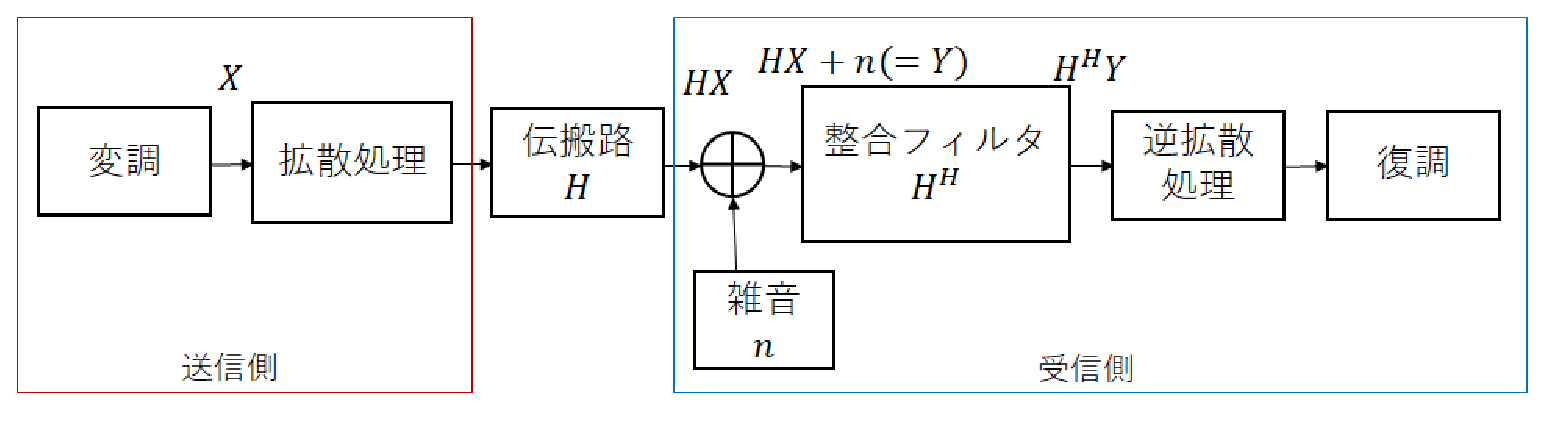
\includegraphics[width=\linewidth]{chapter3/figure/VC.eps}
    \caption{VC概略図}
    \label{figVC}
\end{figure}

\section{PPL(Ping-Pong-Loop)}
従来のVCでは,伝搬路推定を用いて伝搬路行列$\bm{H}$を求めた後,そこから合成チャネル行列
$\bm{H^HH}$を計算し,当該チャネル行列を固有値分解することによって固有値・固有ベクトルを求める.
PPLは,従来の伝搬路推定,固有値分解の演算部分を二つの無線機間のごく単純な往復処理に置き換えた
ものである.
PPLの原理は,行列の固有値・固有ベクトルの導出方法として一般的なべき乗法を基礎とする.
任意ベクトル$\bm{x}$を,二つの無線機間で繰り返し送受信しつつ,各無線機に
おいて簡単な非線形処理を施すことで,徐々にこの任意ベクトル$\bm{x}$を固有ベクトルへと収束させる.
PPLは,伝搬路推定や固有値分解等の膨大な演算をごく単純な非線形処理を含む送受信機間往復に置換する
点を特徴とする.

PPLの例として,無線機Aと無線機B間での反復処理を考える.
ここでは上下回線とも同一周波数を用いる.
半2重通信を想定する.また,伝搬路行列$\bm{H}$は時不変チャネルとし,雑音の影響はないとする.
PPLを大きく分けて,無線機Aから無線機Bへの往路と無線機Bから無線機Aへの復路の二つに分けて説明する.
無線機A,B間の往復によって,任意ベクトル$\bm{x}$が合成チャネル行列$\bm{H^H}$を通過したと
見做すことができれば,2.3節で解説したべき乗法のアルゴリズムによって伝搬路推定を用いることなく
固有値・固有ベクトルを求めることが可能になる.
図\ref{figPPL}にPPLの概略図を示す.

\begin{figure}
    \centering
    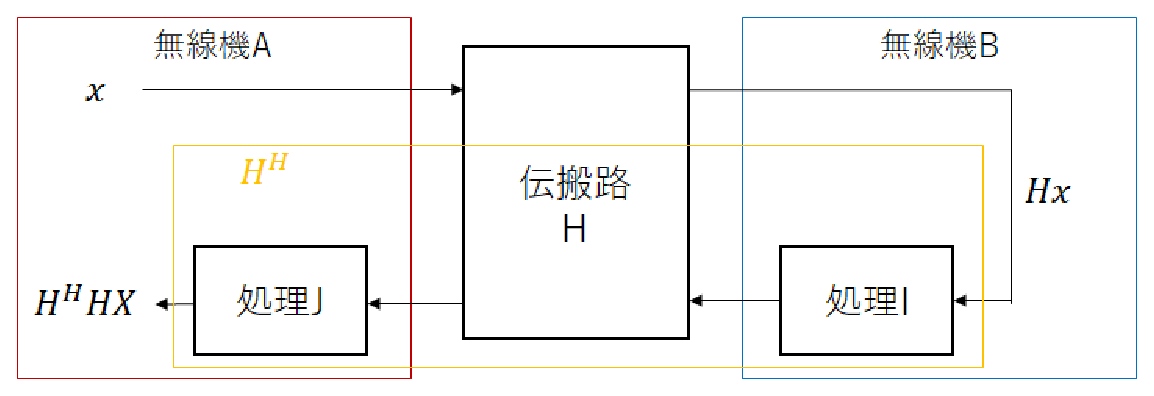
\includegraphics[width=\linewidth]{chapter3/figure/PPL.eps}
    \caption{PPL概略図}
    \label{figPPL}
\end{figure}

まず,往路について,無線機Aから任意ベクトル$\bm{x}$を送信する.当該ベクトルは伝搬路$\bm{H}$を
通過し,無線機Bの受信端にて$\bm{Hx}$として受信される.
次に,復路について,$\bm{Hx}$を無線機Aへと伝送するが,この時,復路の伝搬路が$\bm{H^H}$と
等価となるように,伝送の前後に非線形処理Iと非線形処理Jの二つを挿入する.
これによって,無線機A,B間を反復することで,見かけ上,任意ベクトル$\bm{x}$が
合成チャネル行列$\bm{H^HH}$を通過したと見做すことができるようになる.
一連の反復処理を複数回繰り返すことで,べき乗法の原理に基づいて任意ベクトル$\bm{x}$は徐々に
固有ベクトルに収束していき,その過程で固有値も求めることができる.

\section{復路のチャネルを$H^H$と見做すための非線形処理}
本節では,3.2節で述べた復路のチャネルを$\bm{H^H}$と見做すための非線形処理I,Jについて説明する.
図 \ref{figPPL}が示すように,無線機Aの非線形処理を処理J,無線機Bの非線形処理を処理Iとする.
具体的に,非線形処理I,Jによって,どのようにして合成チャネル行列$\bm{H^HH}$を通過したと見做せるか
解説する.
説明に当たって,以下では$N=3$の任意ベクトル$\bm{x}$,パス数$K=3$の$\bm{H}$を考える.
図 \ref{figProcI}と図 \ref{figProcJ}にそれぞれ処理I、処理Jの手順を示す.

\begin{figure}
    \centering
    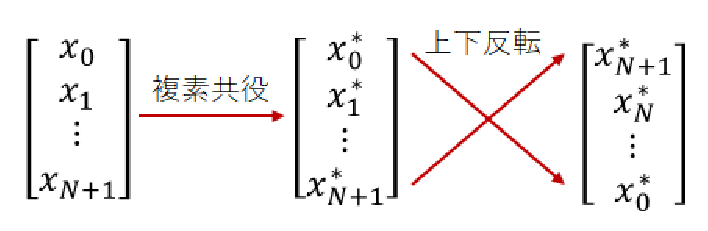
\includegraphics[width=0.6\linewidth]{chapter3/figure/ProcI.eps}
    \caption{処理I}
    \label{figPPL}
\end{figure}
\begin{figure}
    \centering
    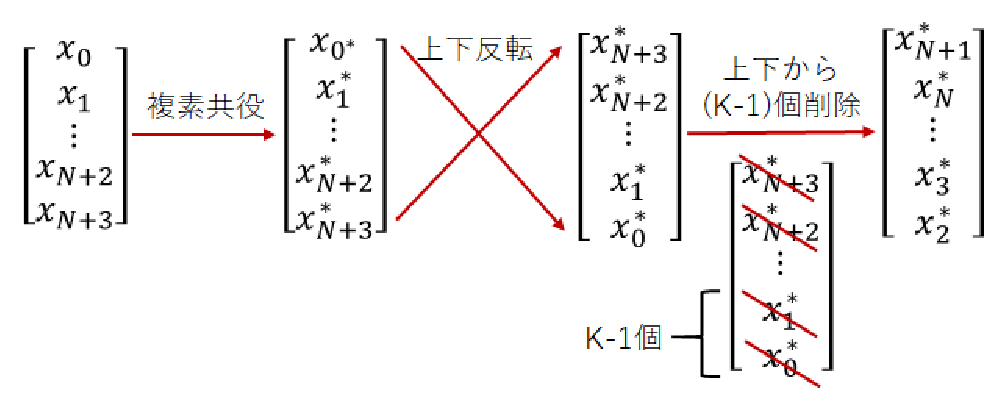
\includegraphics[width=0.7\linewidth]{chapter3/figure/ProcJ.eps}
    \caption{処理J}
    \label{figPPL}
\end{figure}

図 \ref{figProcI}に示している通り,処理Iはベクトルの複素共役をとった後,上下を反転させる.
また,処理Jは図 \ref{figProcJ}にあるように途中まで処理Iと同じプロセスとなっているが,これに
加えて最後にベクトルの上下から(K-1)個分の要素を除去する処理が追加されている.

次に,処理I,処理Jを施すことでどのようにして復路を$\bm{H^H}$と見做せるようになるのかを具体例を
使って説明する.
説明に当たって,伝送する任意ベクトル$\bm{x}$,伝搬路行列$\bm{H}$は以下を考える.

\begin{equation}
    \bm{x} = \left[
        \begin{array}{c}
            x_0 \\
            x_1 \\
            x_2
        \end{array}
    \right]
\end{equation}

\begin{equation}
    \bm{H} = \left[
        \begin{array}{ccc}
            h[0] & 0 & 0 \\
            h[1] & h[0] & 0 \\
            h[2] & h[1] & h[0] \\
            0 & h[2] & h[1] \\
            0 & 0 & h[2]
        \end{array}
    \right]
\end{equation}

まず,$\bm{x}$が無線機Aから無線機Bに向けて伝送される場合を考える.
伝搬路$\bm{H}$を通って無線機Bの受信端で受信されたベクトル$\bm{x^{\prime}}$は,
\begin{equation}
    \bm{x^{\prime}} = \bm{Hx} = \left[
        \begin{array}{c}
            h[0]x_0 \\
            h[1]x_0 + h[0]x_1 \\
            h[2]x_0 + h[1]x_1 + h[0]x_2 \\
            h[2]x_1 + h[1]x_2 \\
            h[2]x_2
        \end{array}
    \right]
    = \left[
        \begin{array}{c}
            x_0^{\prime} \\
            x_1^{\prime} \\
            x_2^{\prime} \\
            x_3^{\prime} \\
            x_4^{\prime}
        \end{array}
    \right]
\end{equation}
となる.このベクトル$\bm{x^{\prime}}$に処理Iを施すと,
\begin{equation}
    \bm{x^{\prime}} = \bm{Hx} = \left[
        \begin{array}{c}
            h[2]^*x_2^* \\
            h[2]^*x_1^* + h[1]^*x_2^* \\
            h[2]^*x_0^* + h[1]^*x_1^* + h[0]^*x_2^* \\
            h[1]^*x_0^* + h[0]^*x_1^* \\
            h[0]^*x_0^*
        \end{array}
    \right]
    = \left[
        \begin{array}{c}
            x_4^{\prime*} \\
            x_3^{\prime*} \\
            x_2^{\prime*} \\
            x_1^{\prime*} \\
            x_0^{\prime*}
        \end{array}
    \right]
\end{equation}
となる.これを復路の伝搬路$\bm{H}$に通すと,無線機Aの受信端で受信されるベクトルは,
\begin{equation}
    \bm{Hx^{\prime*}} \left[
        \begin{array}{c}
            h[0]x_4^{\prime*} \\
            h[1]x_4^{\prime*}+h[0]x_3^{\prime*} \\
            h[2]x_4^{\prime*}+h[1]x_3^{\prime*}+h[0]x_2^{\prime*} \\
            h[2]x_3^{\prime*}+h[1]x_2^{\prime*}+h[0]x_1^{\prime*} \\
            h[2]x_2^{\prime*}+h[1]x_1^{\prime*}+h[0]x_0^{\prime*} \\
            h[2]x_1^{\prime*}+h[1]x_0^{\prime*} \\
            h[2]x_0^{\prime*}
        \end{array}
    \right]
\end{equation}
となり,処理Jを施すと,
\begin{equation}
    \left[
        \begin{array}{c}
            h[2]^*x_2^{\prime}+h[1]^*x_1^{\prime}+h[0]^*x_0^{\prime} \\
            h[2]^*x_3^{\prime}+h[1]^*x_2^{\prime}+h[0]^*x_1^{\prime} \\
            h[2]^*x_4^{\prime}+h[1]^*x_3^{\prime}+h[0]^*x_2^{\prime}
        \end{array}
    \right]
\end{equation}
となる.

次に,無線機Bで受信された$\bm{x^{prime}}$に$\bm{H^H}$をかけたものが,式(3.20)と一致するか
確認する.まず,伝搬路行列$\bm{H}$の随伴行列$\bm{H^H}$は次のようになる.
\begin{equation}
    \bm{H^H} = \left[
        \begin{array}{ccccc}
            h[0]^* & h[1]^* & h[2]^* & 0 & 0 \\
            0 & h[0]^* & h[1]^* & h[2]^* & 0 \\
            0 & 0 & h[0]^* & h[1]^* & h[2]^*
        \end{array}
    \right]
\end{equation}

これを無線機Bで受信された$\bm{x^{\prime}}$に左からかけると,
\begin{equation}
    \bm{H^Hx^{\prime}} = \left[
        \begin{array}{c}
            h[2]^*x_2^{\prime}+h[1]^*x_1^{\prime}+h[0]^*x_0^{\prime} \\
            h[2]^*x_3^{\prime}+h[1]^*x_2^{\prime}+h[0]^*x_1^{\prime} \\
            h[2]^*x_4^{\prime}+h[1]^*x_3^{\prime}+h[0]^*x_2^{\prime}
        \end{array}
    \right]
\end{equation}
となり,これは式(3.20)と一致する.よって,非線形処理IとJを施すことで復路を見かけ上$\bm{H^H}$と
見做せることが確認できた.

\section{合成チャネル行列の第1固有符号導出}
ここではべき乗法を基本原理として,PPLにおいてどのように合成チャネル行列の固有ベクトル・固有値を求めて
いくか解説を行う.まず,3.3節で示したように二つの無線機間で任意ベクトル$\bm{x}$を往復せた時,
非線形処理によって1往復後のベクトルは$\bm{H^HHx}$となる.これによって,べき乗法の
適用が可能になり,2往復目は$\bm{{H^HH}^2x}$となり,複数回

\section{合成チャネル行列の第2固有符号以降導出}
